\chapter{Laser-Induced Fluorescence}
\label{c:laser-induced_fluorescence}

Laser-induced fluorescence is a method of spectroscopy that excites a molecule into a higher electronic state via the absorption of laser radiation. A single ro-vibrational band is isolated and excited. Next, the molecule relaxes back into the original electronics state, filling multiple lower vibrational states in the process. These vibrational states are filled according to the known Franck-Condon factors.

Figure \ref{f:laser-induced_fluorescence_in_iodine} below shows the jump from the ground state to the excited state via laser excitation. Subsequently, the molecule relaxes to fill multiple vibrational states within the original electronic state.

\begin{figure}[H]
    \centering
    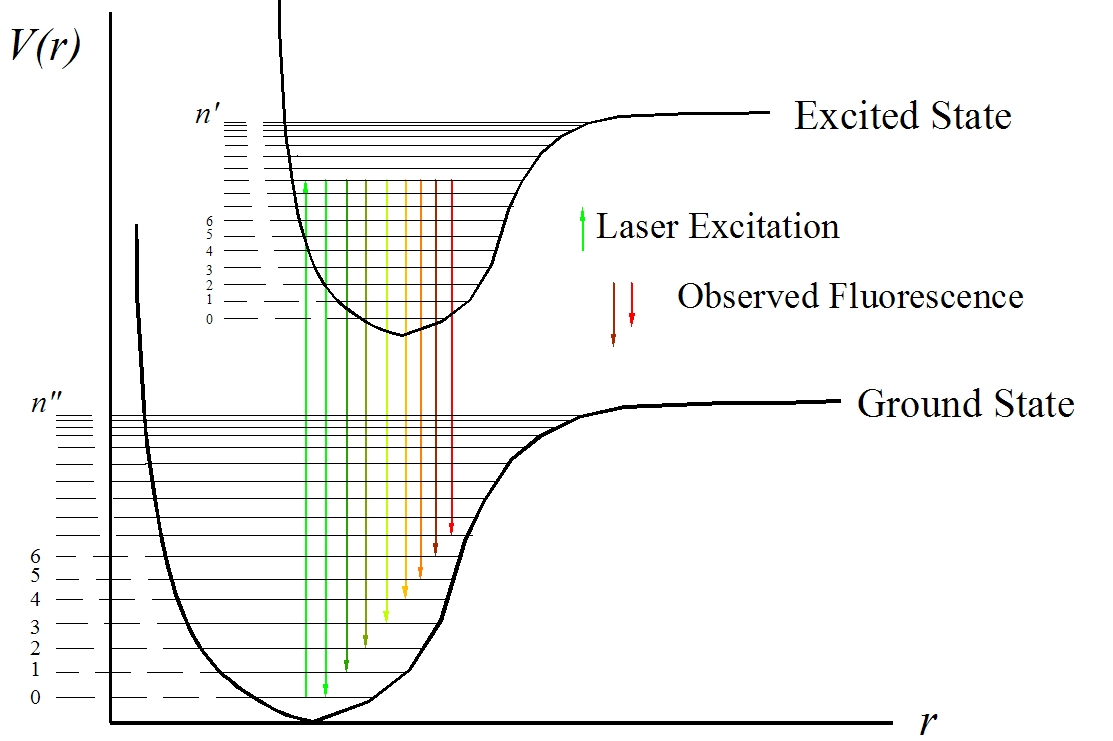
\includegraphics[width=0.8\textwidth]{img/lif_bands}
    \caption{Laser-induced fluorescence in Iodine.}
    \label{f:laser-induced_fluorescence_in_iodine}
\end{figure}
